\begin{figure}[h!]
\centering
\begin{tikzpicture}[scale=1]

% W als Ursprung gewählt
% U und w sind kurzgeschlossen

% V und W beliebig festlegen (als Dreiecksbasis)
\coordinate (1W) at (0, 0);
\coordinate (1V) at (0:12.6);

% Konstruktion primär
\draw[name path=Warc, dotted] (70:12.33) arc [start angle=70, end angle=50, radius=12.33];
\draw[name path=Varc, dotted] ([shift=(1V)] 130:12.6) arc [start angle=130, end angle=110, radius=12.6];
\path[name intersections={of=Warc and Varc,name=1U}];
\coordinate (1U) at (1U-1);
%\coordinate (U1) at (60:12.333);
\coordinate (2U) at (1U);
\coordinate (N) at ($1/3*(1U)+1/3*(1V)+1/3*(1W)$);

% Konstruktion sekundär
\draw[name path=warc, dotted] ([shift=(2U)] -20:8.56) arc [start angle=-20, end angle=-40, radius=8.56];
\draw[name path=uwarc, dotted] ([shift=(2U)] -100:8.1) arc [start angle=-100, end angle=-80, radius=8.1];
\draw[name path=Vuarc, dotted] ([shift=(1V)] 75:6.56) arc [start angle=75, end angle=90, radius=6.56];
\draw[name path=Vvarc, dotted] ([shift=(1V)] 155:6.96) arc [start angle=155, end angle=170, radius=6.96];
\path[name intersections={of=warc and Vuarc,name=2V}];
\path[name intersections={of=uwarc and Vvarc,name=2W}];
\coordinate (2V) at (2V-1);
\coordinate (2W) at (2W-1);
%\coordinate (n) at ($1/3*(2V)+1/3*(2W)+1/3*(2U)$);

% Punkte
\draw (N) node[anchor=south east, outer sep=3pt] {N};
\draw (1U) node[anchor=south, outer sep=5pt] {1U, 2U};
\draw (1V) node[anchor=north west] {1V};
\draw (1W) node[anchor=north east] {1W};
\draw (2V) node[anchor=west,label={[shift={(0.3,-0.8)}]2V}] {};
\draw (2W) node[anchor=north] {2W};

% Verbindungen und Spannungspfeile
\draw[gray] (1V) -- (1W);
\draw[gray] (1W) -- (1U);
\draw[gray] (1U) -- (1V);
\draw[->,name path=UN] (1U) -- (N);
\draw[->] (1V) -- (N);
\draw[->] (1W) -- (N);
\draw[->] (2V) -- (2W);
\draw[->] (2W) -- (2U);
\draw[->] (2U) -- (2V);

% Kreisbogenbeschriftungen
\draw[<-] ([shift=(2U)] -35:8.56) -- ([shift=(2U)] -35:9.06) node[anchor=west] {$U_\mathrm{1U2V}$};
\draw[<-] ([shift=(2U)] -80:8.1) -- ([shift=(2U)] -80:8.6) node[anchor=north] {$U_\mathrm{1U2W}$};
\draw[<-] ([shift=(1V)] 88:6.56) -- ([shift=(1V)] 88:7.06) node[anchor=south] {$U_\mathrm{1V2V}$};
\draw[<-] ([shift=(1V)] 168:6.96) -- ([shift=(1V)] 168:7.46) node[anchor=south] {$U_\mathrm{1V2W}$};
\draw[<-] ([shift=(1V)] 128:12.6) -- ([shift=(1V)] 128:13.1) node[anchor=south] {$U_\mathrm{1U1V}$};
\draw[<-] ([shift=(1W)] 68:12.33) -- ([shift=(1W)] 68:12.83) node[anchor=south] {$U_\mathrm{1W1U}$};

% Schieflaststrom
\coordinate (ILast) at ($(2W)!0.1*85.5cm!(2V)$);
\draw[->, red] (2W) -- (ILast) node[anchor=west] {$I_\mathrm{Last}$};

% Strom Primärseite
\coordinate (IU) at ($(N)!-0.1*41.1cm!(1U)$);
\coordinate (IVhelp) at ($(N)!-0.1*27.2cm!(1V)$);
\coordinate (IV) at ($(IU)-(N)+(IVhelp)$);
\coordinate (IWhelp) at ($(N)!-0.1*68.1cm!(1W)$);
\coordinate (IW) at ($(IV)-(N)+(IWhelp)$);
%\draw[->, red] (N) -- (IU) node [anchor=north west] {$I_{1U}$};
%\draw[->, red] (N) -- (IVhelp) node [anchor=north east] {$I_{1V}$};
%\draw[->, red] (N) -- (IWhelp) node [anchor=north] {$I_{1W}$};

% Stundenziffer (ausgeblendet)
%\begin{scope}
%\draw[name path=un] (u) -- ($(n)!-0.6!(u)$);
%\path[name intersections={of=UN and un,name=helper}];
%\coordinate (helper) at (helper-1);
%\path[clip] (U) -- (helper) -- (u) -- cycle;
%\draw (helper) circle (0.8);
%\draw (helper) node[anchor=south west] {\SI{90}{\degree}};
%\end{scope}

\end{tikzpicture}
\caption{Zeigerdiagramm zum Schieflastversuch}
\label{fig:zeigerdiagramm_schieflast}
\end{figure}

\begin{figure}[h!]
\centering
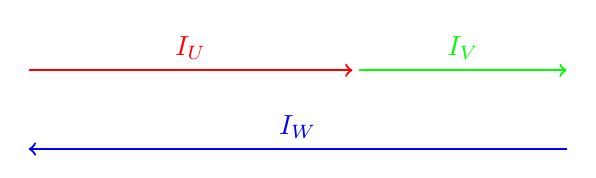
\begin{tikzpicture}[scale=1]

\draw[->, red, thick] (0,0) -- (4.11,0) node [midway,above] {$I_{U}$};
\draw[->, green, thick] (4.2,0) -- (6.83,0)node [midway,above] {$I_{V}$};
\draw[->, blue, thick] (6.83,-1) -- (0,-1)node [midway,above] {$I_{W}$};

\end{tikzpicture}
\caption{Zeigerdiagramm der Ströme auf der Primärseite}
\label{fig:zeigerdiagramm_pri_stroeme}
\end{figure}